%***************************************PREAMBLE***************************************
\documentclass[a4paper,12pt]{article}

\usepackage[utf8]{inputenc}
\usepackage[margin=0.7in]{geometry}
\usepackage[T1]{fontenc}
\usepackage{graphicx}
\usepackage{float}
\usepackage{setspace}
\usepackage{appendix}

%***************************************DOCUMENT***************************************

\begin{document}
	\fontfamily{ptm}\selectfont
	%%%%%%%%%%%%%%%%%%%%%%%%%%%%%%%%%%%%%%%COVERSHEET%%%%%%%%%%%%%%%%%%%%%%%%%%%%%%%%%%%%%%%
	\begin{titlepage}
		\setlength{\voffset}{-0.8in}
		\noindent \makebox[\textwidth]{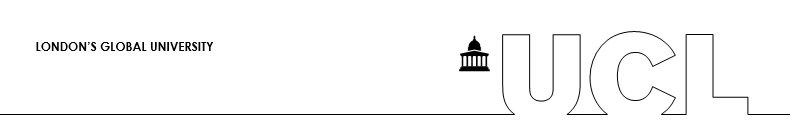
\includegraphics[width=1.2\textwidth]{images/Coversheet_Header.png}}
	
			\vspace{15mm}
			
			\begin{center}
				{\Huge \textbf{COMP0037 \\ \vspace{10mm} Report}}
			
				\vspace{8mm}
			
				\begin{spacing}{1.8}
					{\huge Path Planning in a Known World}
				\end{spacing}
		
			
				\vspace{12mm}
			
				{\LARGE \textbf{Group AS}}
				
				\vspace{10mm}
				
				\begin{tabular}{ll}
					\underline{\textbf{Student Name}}  & \hspace{4mm} \underline{\textbf{Student number}} \vspace{2mm} \\
					Arundathi Shaji Shanthini & \hspace{4mm} 16018351 \\ 
					Dmitry Leyko & \hspace{4mm}  16021440\\ 
					Tharmetharan Balendran & \hspace{4mm} 17011729\\ 
				\end{tabular}
				
				\vspace{13mm}
				
				\begin{tabular}{ll}
					\textbf{Department:} &  Department of Electronics and Electrical Engineering\\ \vspace{3mm}
					\textbf{Submission Date:} &  25\textsuperscript{th} of February 2020
				\end{tabular}
			\end{center}
	\end{titlepage}
	%%%%%%%%%%%%%%%%%%%%%%%%%%%%%%%%%%%%%%
	
	\pagebreak
	
	\tableofcontents
	
	\pagebreak
	
	%%%%%%%%%%% PART 1 %%%%%%%%%%%%%%%%%
	\section{Implement and Investigate Properties of Path Planning Algorithms}
		
	\subsection{Path Planning Algorithms}
			
			\begin{figure}[H]
				\renewcommand\thefigure{1.1}
				\centering
				
				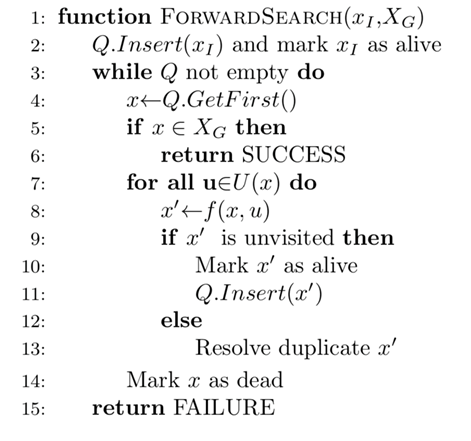
\includegraphics[scale=0.6]{images/general_forward_search_pseudocode.png}
				\caption{The general forward search algorithm pseudocode. }
			\end{figure}
			
			All of the path planning algorithms have the same backbone and can be summed up into 15 lines of pseudocode shown in Fig 1.1. This algorithm describes the process of finding a path from a cell ($x_I$) to a goal cell ($X_G$). This general algorithm is called the general forward search algorithm and is implemented in the \textbf{GeneralForwardSearchAlgorithm} class. All planners that are implemented inherit from this class through the \textbf{CellBasedForwardSearch} class. The search algorithm is similar for all the planners and has also been implemented in the same \textbf{GeneralForwardSearchAlgorithm} class. What differs between the planners is the type of queue that is used and the implementation of the \textbf{resolveDuplicate} function. These properties and functions are defined in the classes of each of the individual planners. The high-level working of the planners we implemented and their properties are described below.
			
			\subsubsection{FIFO - Breadth First Search}

				This algorithm works by selecting a particular node and exploring its neighbours first. It would then pivot around those neighbours to explore each of their neighbours. Layer by layer it will explore all the nodes on the graph network until it reaches the goal. The next nodes to be considered are chosen by first considering the node directly underneath and then considering the neighbouring nodes going anti-clockwise. This way of allocating the next set of nodes to be considered, is the same for all algorithms. The Breadth First Algorithm uses a queue to keep track of the order of the exploration in the network. If a particular node shows itself twice to the algorithm, it will use the first instance of it ignoring the second. The first path that reaches the finishing node is the final output path, no mater of the cost. The name First in First Out (FIFO) comes from the type of queue implemented in this search algorithm. The next node to be considered at any point is the one that was added the first out of all the nodes in the queue.
				\\
				The Breadth First Search Algorithm utilizes a normal unsorted queue and was 
				\\
				The biggest advantage of FIFO is that it will never get stuck in a blind alley. If there is a solution it will find it. If there are multiple solutions, it will find one with the least steps. The memory usage can be large as it stores all the nodes that it visits. If the solution is far, it might take a lot of time to find, as well as that the FIFO algorithm does not guarantee optimality.
				\\
				In the worst case scenario with the FIFO algorithm will consider every possible node and edge. Therefore the complexity can be expressed as O(N+E) where N is the total number of nodes and E is the total number of edges in the graph. 
			
			\subsubsection{LIFO - Depth First Search}
			
				This algorithm works by selecting a particular node and exploring its neighbour at random. It 
				would then perform the same exploration on the neighbour and will pick a random neighbour of its. 
				This will continue until it either riches a node with no other neighbours or visits an already 
				visited node, it will then backtrack until it gets to a node with an unvisited neighbours, and 
				it will explore that particular branch off. Once it backtracks to the original node and it has 
				no other neighbours to explore, the algorithm would have finished and visited every node in the 
				graph. The first path that reaches the finishing node is the final output path, no mater of the 
				cost. 
				\\
				The advantage of DFA is the linear memory usage. It will also be faster than BFA, however will
				produce a worse solution then it.  The biggest disadvantage is that there could be cases where 
				it does not produce solutions. 
				\\
				Similarly to the Breadth First Algorithm, in the worst case scenario the Depth first algorithm
				will consider each node of the graph. This means that once again the complexity of the algorithm
				can be expressed as O(N+E) where N is the total number of nodes and E is the total number of edges
				in the graph
			
			\subsubsection{Greedy Search}
				The Greedy Search Algorithm starts at the first node and adds neighbouring nodes to the queue. The
				type of queue used in this algorithm is a priority queue with the priority value being the euclidean
				distance between the node and the goal. This means that the nodes in the queue are sorted by their
				euclidean distance to the goal. As a result when a node is popped from the queue it will be the node
				with the lowest euclidean distance to the goal (out of the nodes in the queue). As a result the algorithm
				will consider the cells closer to the goal first.
				\\
				The biggest advantage of the greedy algorithm is its easy implementation and its efficiency in simple
				cases. In maps with minimal/no obstructions, the greedy algorithm is able to find a path with significantly
				fewer cells visited. However the optimality of the path is not guaranteed.
				\\
				Put time comp here!!!
			\subsubsection{Dijkstra's}
				This algorithm works by first setting the values for distances to every node to infinity. Once the
				starting node is specified, its distance value is set to zero. The algorithm then explores the neighbours 
				of the starting node and records the distance to each. Once this is done, the algorithm will then pivot
				on the most promising node (the node which has the shortest distance from the previous one, exploring
				its neighbours. If it finds that there is a shorter path to a node that it has found distance to before,
				it will replace the old distance with the new one and record the new path to it. Once it reaches the
				target node with the shortest distance possible it will mark that path as the optimal one. 
				\\
				Dijkstra's will always find the shortest path. It may however take a much longer time to do so as it
				performs blind search thus exploring nodes that go away from the goal node. 
				\\
				This search runs in a time complexity of O(E*log(V)), where V are vertices and E are edges. 
			\subsubsection{A* Search}
				This algorithm works in a similar way to dijkstara’s however it additionally uses a heuristic to affect
				the way it selects which nodes to explore and visit. Heuristics used in our assignments are: 1. A
				non-negative constant value c, 2. The Euclidean Distance to the goal, 3. The Octile Distance to the goal
				and 4. Manhattan Distance to the goal. Each node gets assigned a heuristic value. When the algorithm starts,
				the starting node is specified. The algorithm then explores its neighbours of the selected node. It ads them
				to the queue in the order of the combined value of distance from to start and heuristic. The algorithm will
				then move onto exploring from the node that is first in the queue. It will add the neighbours of that node
				into the same queue based on the combined parameter. If the algorithm visits a node which has already been
				visited, it will compare the travel distances from the start and ignore the heuristic value to select which
				path is best and editing the entry in the queue. Once the node and all its connections are fully explored,
				it is removed from the queue. Once the algorithm finds the target node, it has found the shortest path to it. 
				\\
				A* algorithm can also be adjusted by weighing the huristic in the addative cost. This will adjust the way
				that A* search making it more inadmissable .
				\\
				A* has a massive advantage over other algorithms which is the weighting of the nodes which allows the algorithm
				also consider distance to the target in deciding where to move to. This allows the algorithm to prioritise the
				queue based on the heuristic. 
				\\
				Put time comp here!!!
			\subsection{Comparing Performance of Algorithms}

		Describe the metrics used to compare performance \\
		Descirbe how they were implemented \\
		Compare and explain the difference in performance of the algorithms (See Teams for more details)


	%%%%%%%%%%%%%%%%%%%%%%%%%%%%%%%%%%%%%%
	%%%%%%%%%%% PART 2 %%%%%%%%%%%%%%%%%
	\section{Implementation in ROS}
	controller 
	- Improved on P
	- Considered PID 
	- Considered reducing the number of waypoints to make controlling better 
	- Sampling rate can be a factor 
	%%%%%%%%%%%%%%%%%%%%%%%%%%%%%%%%%%%%%%
	
	\newpage
	
	\appendix
	\appendixpage
	\addappheadtotoc
	\section{Class Inheritance}
	\subsection{Planner Inheritance}
	\label{appendix:planner}
	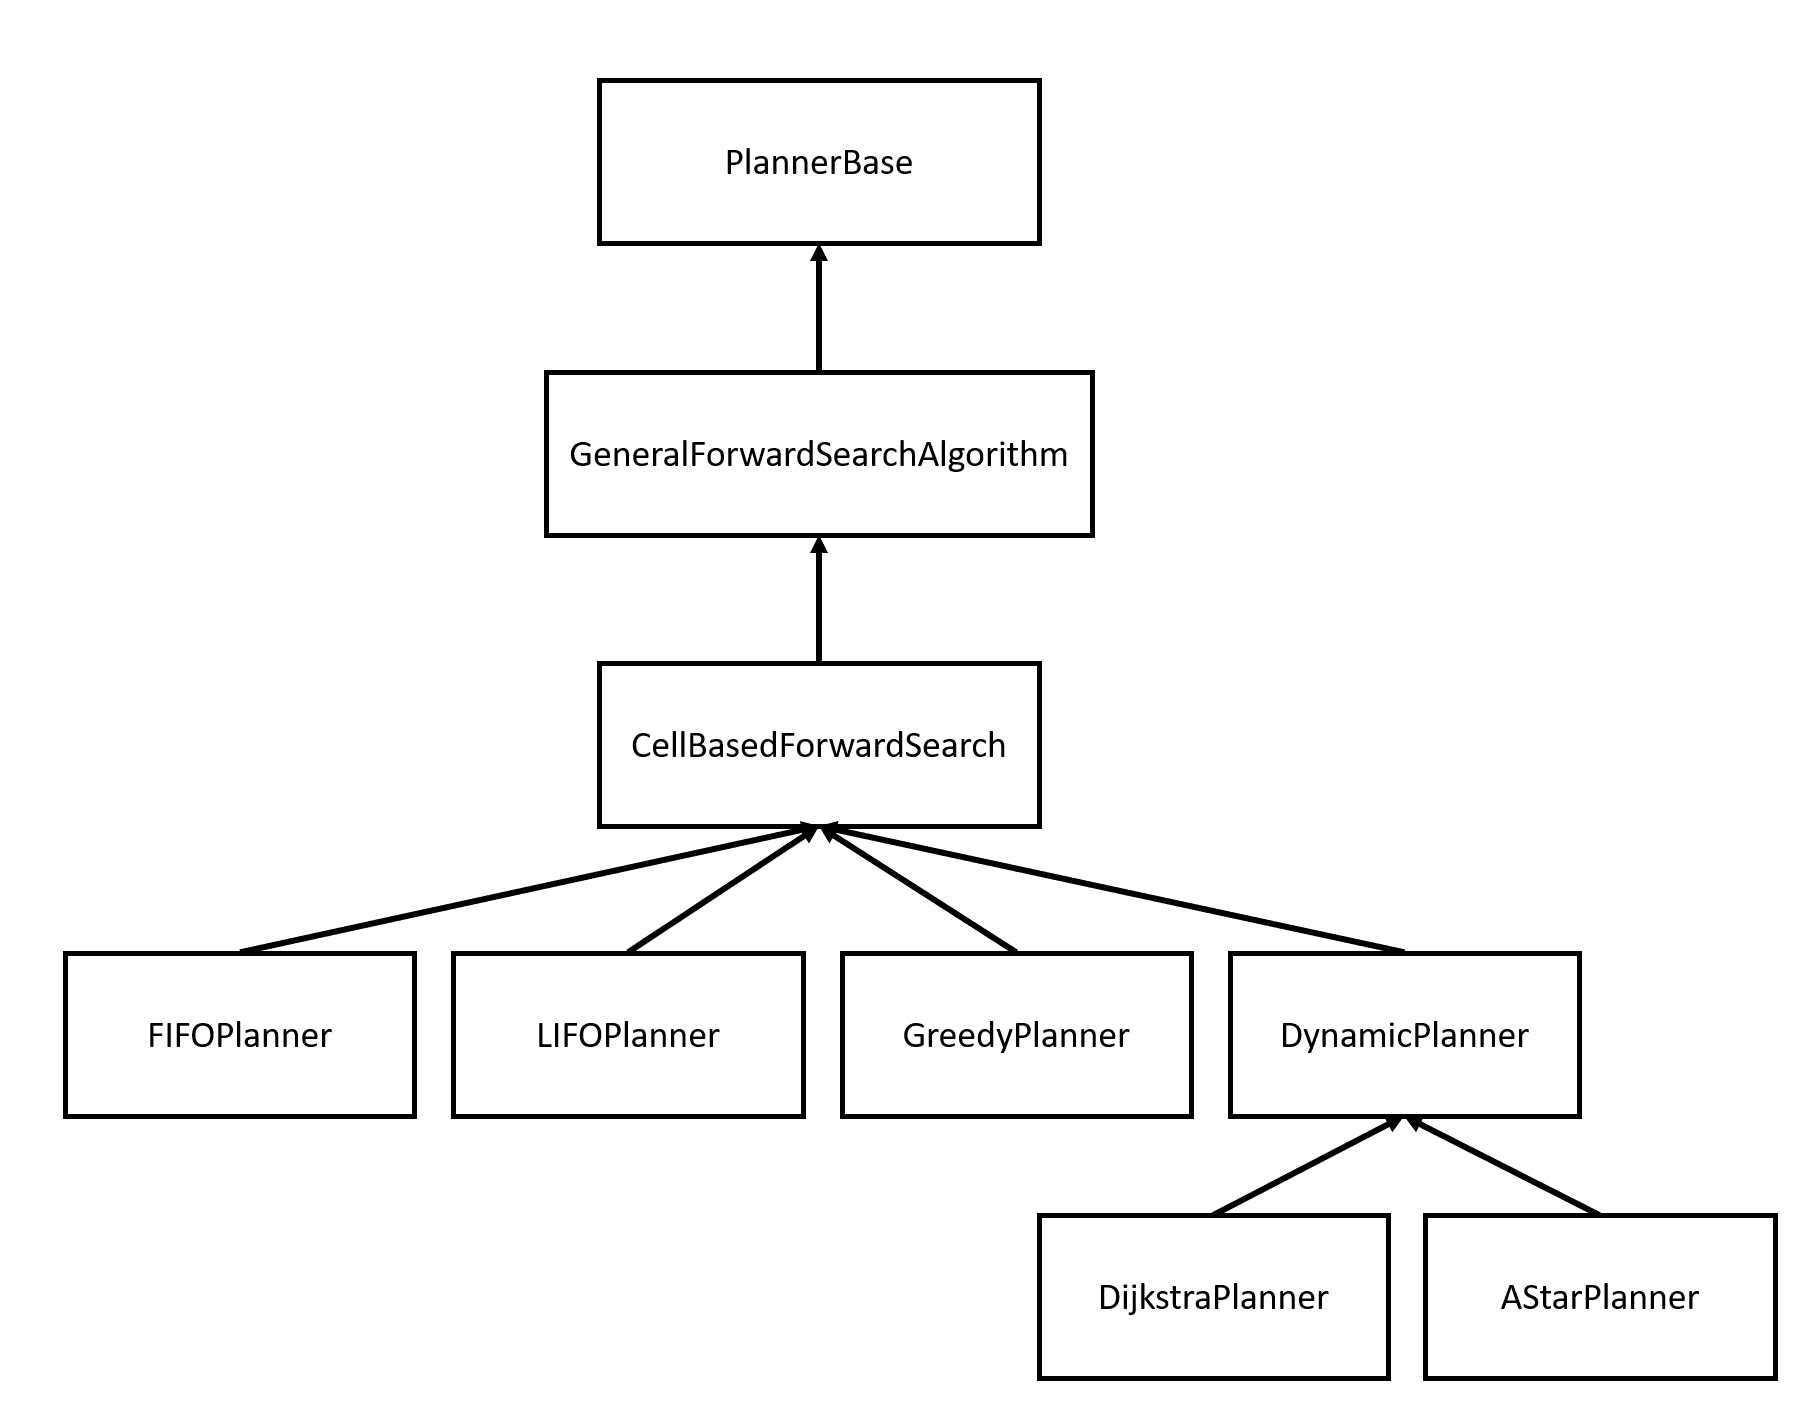
\includegraphics[scale=0.6]{images/planner_inheritance.png}
	\subsection{Controller Inheritance}
	\label{appendix:controller}
	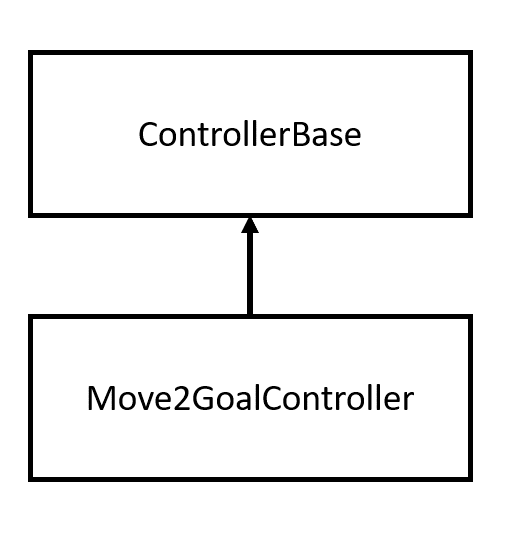
\includegraphics[scale=0.6]{images/controller_inheritance.png}
	
\end{document}